\documentclass[12pt]{article}
\usepackage{graphicx,import}
\usepackage[svgnames]{xcolor} 
\usepackage{fancyhdr}
\usepackage{subfig}
\usepackage{hyperref}
\usepackage{enumitem}
\usepackage[many]{tcolorbox}
\usepackage{listings}
\usepackage[a4paper, total={6in, 8in} , bottom = 25mm , top = 25mm, headheight = 1.25cm , includehead,includefoot,heightrounded ]{geometry}
\usepackage{afterpage}
\usepackage{amssymb}
\usepackage{pdflscape}
\usepackage{gensymb}
\usepackage{textcomp}
\usepackage{tikz,pgfplots}
\usepackage{xecolor}
\usepackage{rotating}
\usepackage{pdfpages}
\usepackage[T1]{fontenc}
\usepackage{tikz}
\usepackage[utf8]{inputenc}
\usepackage{PTSerif} 
\usepackage{seqsplit}
\usepackage{fancyvrb}
\usepackage{mips}
\usepackage{multirow}
\usepackage{hhline}
\usepackage[edges]{forest}
\usepackage{tabularx}
\usepackage{float}
\usepackage{graphicx}
\usepackage{cprotect}
\usepackage{url}
\usepackage{listings}
\usepackage{xcolor}
\usepackage{pifont}
\newcommand{\xmark}{\ding{55}}%
\def\checkmark{\tikz\fill[scale=0.4](0,.35) -- (.25,0) -- (1,.7) -- (.25,.15) -- cycle;}

\hypersetup{
	colorlinks   = true, %Colours links instead of ugly boxes
	urlcolor     = blue, %Colour for external hyperlinks
	linkcolor    = blue, %Colour of internal links
	citecolor   = red %Colour of citations
}

\definecolor{codegreen}{rgb}{0,0.6,0}
\definecolor{codegray}{rgb}{0.5,0.5,0.5}
\definecolor{codepurple}{rgb}{0.58,0,0.82}
\definecolor{backcolour}{rgb}{0.95,0.95,0.92}
\definecolor{mGreen}{rgb}{0,0.6,0}
\definecolor{mGray}{rgb}{0.5,0.5,0.5}
\definecolor{mPurple}{rgb}{0.58,0,0.82}
\definecolor{backgroundColour}{rgb}{0.95,0.95,0.92}

\NewDocumentCommand{\codeword}{v}{
	\texttt{\textcolor{blue}{#1}}
}
\lstset{language=java,keywordstyle={\bfseries \color{blue}}}
\definecolor{dkgreen}{rgb}{0,0.6,0}
\definecolor{gray}{rgb}{0.5,0.5,0.5}
\definecolor{mauve}{rgb}{0.58,0,0.82}



\lstdefinestyle{mystyle}{
	backgroundcolor=\color{backcolour},   
	commentstyle=\color{codegreen},
	keywordstyle=\color{magenta},
	numberstyle=\tiny\color{codegray},
	stringstyle=\color{codepurple},
	basicstyle=\ttfamily\normalsize,
	breakatwhitespace=false,         
	breaklines=true,                 
	captionpos=b,                    
	keepspaces=true,                 
	numbers=left,                    
	numbersep=5pt,                  
	showspaces=false,                
	showstringspaces=false,
	showtabs=false,                  
	tabsize=2
}

\lstdefinestyle{CStyle}{
	backgroundcolor=\color{backgroundColour},   
	commentstyle=\color{mGreen},
	keywordstyle=\color{magenta},
	numberstyle=\tiny\color{mGray},
	stringstyle=\color{mPurple},
	basicstyle=\footnotesize,
	breakatwhitespace=false,         
	breaklines=true,                 
	captionpos=b,                    
	keepspaces=true,                 
	numbers=left,                    
	numbersep=5pt,                  
	showspaces=false,                
	showstringspaces=false,
	showtabs=false,                  
	tabsize=2,
	language=C
}



\lstset{ %
	language=[mips]Assembler,       % the language of the code
	basicstyle=\footnotesize,       % the size of the fonts that are used for the code
	numbers=left,                   % where to put the line-numbers
	numberstyle=\tiny\color{gray},  % the style that is used for the line-numbers
	stepnumber=1,                   % the step between two line-numbers. If it's 1, each line
	% will be numbered
	numbersep=5pt,                  % how far the line-numbers are from the code
	backgroundcolor=\color{white},  % choose the background color. You must add \usepackage{color}
	showspaces=false,               % show spaces adding particular underscores
	showstringspaces=false,         % underline spaces within strings
	showtabs=false,                 % show tabs within strings adding particular underscores
	frame=single,                   % adds a frame around the code
	rulecolor=\color{black},        % if not set, the frame-color may be changed on line-breaks within not-black text (e.g. commens (green here))
	tabsize=4,                      % sets default tabsize to 2 spaces
	breaklines=true,                % sets automatic line breaking
	breakatwhitespace=false,        % sets if automatic breaks should only happen at whitespace
	% also try caption instead of title
	keywordstyle=\color{blue},          % keyword style
	commentstyle=\color{dkgreen},       % comment style
	stringstyle=\color{mauve},         % string literal style
	escapeinside={\%*}{*)},            % if you want to add a comment within your code
	morekeywords={*,...}               % if you want to add more keywords to the set
}

\setmainfont[ExternalLocation=fonts/]{EBGaramond-Regular.ttf}


\newenvironment{changemargin}[2]{%
	\begin{list}{}{%
			\setlength{\topsep}{0pt}%
			\setlength{\leftmargin}{#1}%
			\setlength{\rightmargin}{#2}%
			\setlength{\listparindent}{\parindent}%
			\setlength{\itemindent}{\parindent}%
			\setlength{\parsep}{\parskip}%
		}%
		\item[]}{\end{list}}


\definecolor{foldercolor}{RGB}{124,166,198}

\tikzset{pics/folder/.style={code={%
			\node[inner sep=0pt, minimum size=#1](-foldericon){};
			\node[folder style, inner sep=0pt, minimum width=0.3*#1, minimum height=0.6*#1, above right, xshift=0.05*#1] at (-foldericon.west){};
			\node[folder style, inner sep=0pt, minimum size=#1] at (-foldericon.center){};}
	},
	pics/folder/.default={20pt},
	folder style/.style={draw=foldercolor!80!black,top color=foldercolor!40,bottom color=foldercolor}
}

\forestset{is file/.style={edge path'/.expanded={%
			([xshift=\forestregister{folder indent}]!u.parent anchor) |- (.child anchor)},
		inner sep=1pt},
	this folder size/.style={edge path'/.expanded={%
			([xshift=\forestregister{folder indent}]!u.parent anchor) |- (.child anchor) pic[solid]{folder=#1}}, inner xsep=0.6*#1},
	folder tree indent/.style={before computing xy={l=#1}},
	folder icons/.style={folder, this folder size=#1, folder tree indent=3*#1},
	folder icons/.default={12pt},
}

\begin{document}
	
	
	%%% title pages
	\begin{titlepage}
		\begin{center}
			
			\vspace*{0.7cm}
			
			\includegraphics[width=0.4\textwidth]{sharif1.png}\\
			\vspace{0.5cm}
			\textbf{ \Huge{Multicore Computing} }\\
			\vspace{0.5cm}
			\textbf{ \Large{ Assignment Five (Practical)} }
			\vspace{0.2cm}
			
			
			\large \textbf{Department of Computer Engineering}\\\vspace{0.2cm}
			\large   Sharif University of Technology\\\vspace{0.2cm}
			\large   Spring 2022 \\\vspace{0.2cm}
			\noindent\rule[1ex]{\linewidth}{1pt}
			Lecturer:\\
			\textbf{{Dr. Falahati}}
			
			
			\vspace{0.15cm}
			Name - Student Number:\\
			
			\textbf{{Saba Hashemi - 97100581}}\\
			
			\textbf{{Amirmahdi Namjoo - 97107212}}
		\end{center}
	\end{titlepage}
	%%% title pages
	
	
	%%% header of pages
	\newpage
	\pagestyle{fancy}
	\fancyhf{}
	\fancyfoot{}
	\cfoot{\thepage}
	\chead{ Amirmahdi Namjoo - Saba Hashemi}
	\rhead{\includegraphics[width=0.1\textwidth]{sharif.png}}
	\lhead{Assignment Five}
	%%% header of pages
	
	
	

	\section{Question Three}
	
	
The code for this question is included in \Verb+cpu.cpp+, \Verb+cuda-1.cu+, and \Verb+cuda-2.cu+.

The cpu.cpp part uses only CPU instructions and does not use CUDA. The other two both use CUDA. the First one initializes the kernel with parameters \verb+<<<1,1>>>+, but the second one uses

\begin{lstlisting}[language=c++]
	
	int blockSize = 256;
	int numBlocks = (total_size + blockSize - 1) / blockSize;
	
\end{lstlisting}

and calls the kernel with \verb+<<<numBlocsk,blockSize>>>+.

All the codes measure the run time of code and output them in stdout.


The code's main logic is to subtract each pixel's value from $255$. Therefore the main kernel will be as follows:

\begin{lstlisting}[language=c++]
	__global__
	void invert(uchar *image, uchar *inverted_image, size_t total_size) {
		int pixel = blockDim.x * blockIdx.x + threadIdx.x;
		if (pixel < total_size)
		inverted_image[pixel] = 255 - image[pixel];
	}
\end{lstlisting}

You can see the original picture and its inverted result below:


\begin{figure}[H]
	\centering
	\includegraphics[width=0.4\textwidth]{./images/Q3/pic3.jpg}	
	\cprotect\caption{Original Image}
	\label{fig:2-1}
\end{figure}

\begin{figure}[H]
	\centering
	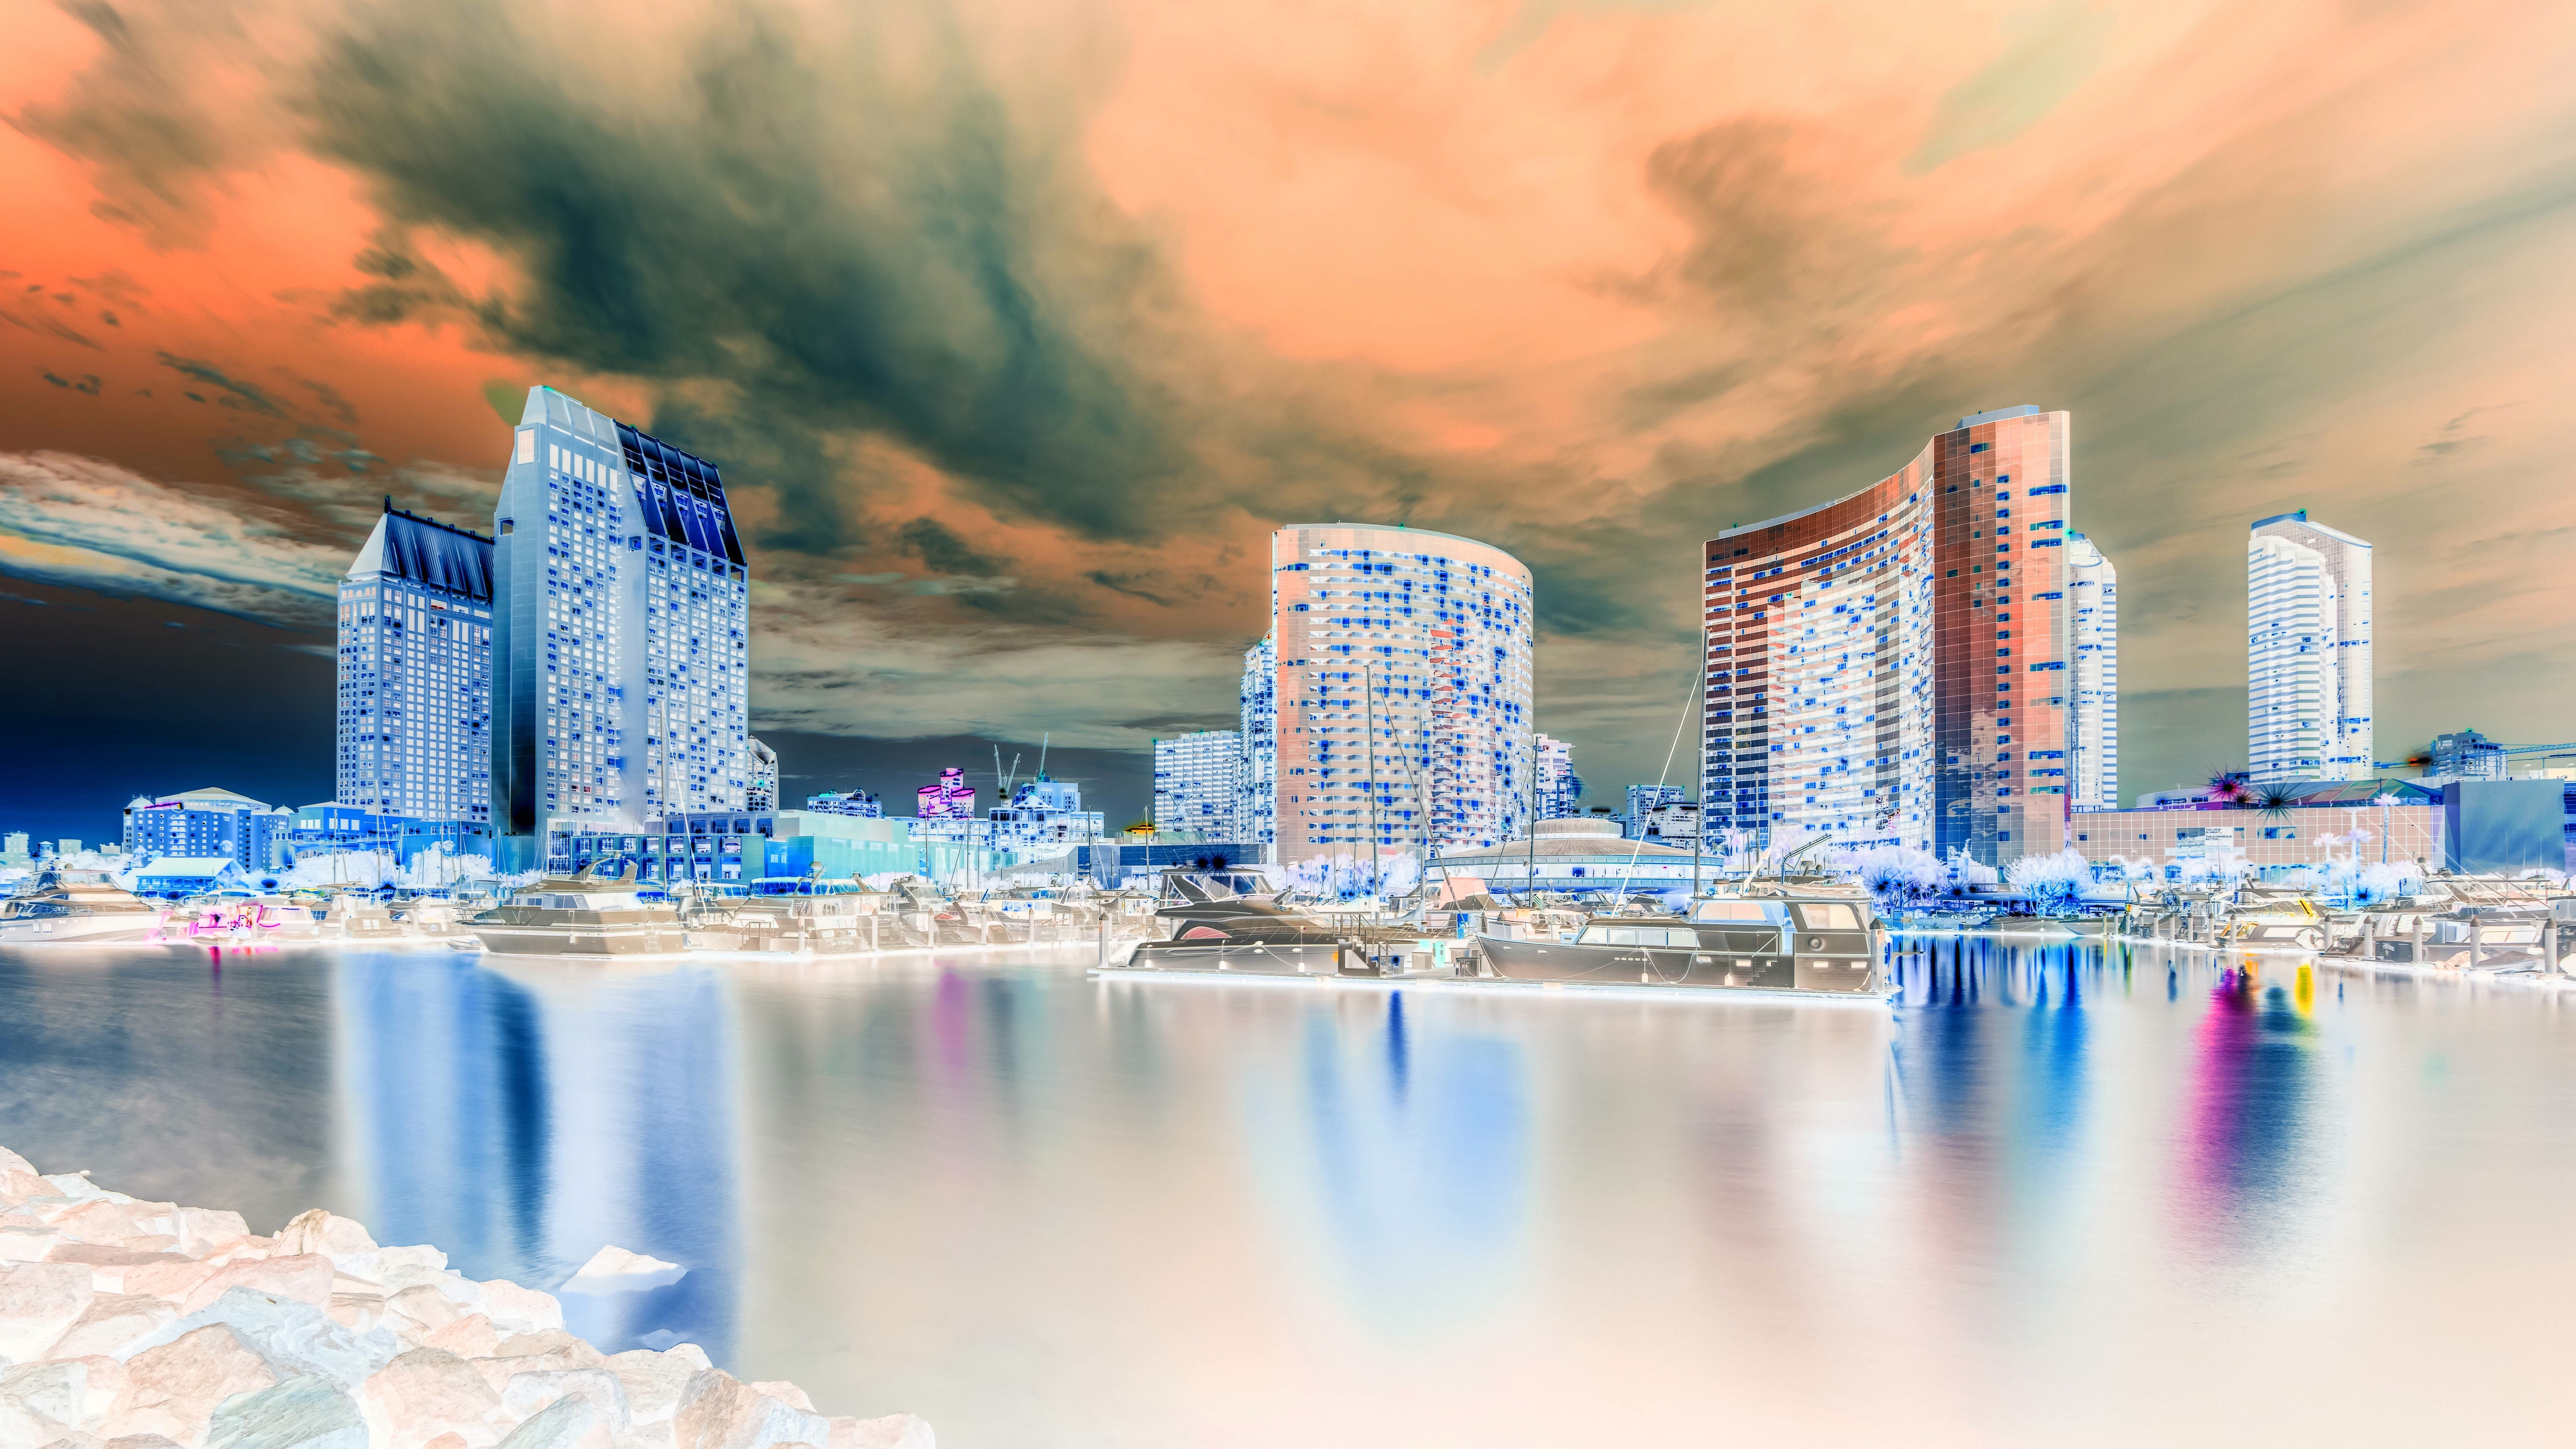
\includegraphics[width=0.4\textwidth]{./images/Q3/out.jpg}	
	\cprotect\caption{Inverted Image}
	\label{fig:2-2}
\end{figure}


\newpage

\section{Question Four}



\newpage

\section{Question Five}

Note: All parts are run on Intel Core i9 11980HK with eight physical cores and 16 logical cores. The results on 16 threads may vary (and show less performance) on systems with less than 16 logical cores. All CUDA parts are run on NVIDIA RTX 3080 Mobile with Compute Capability of 8.6.

\begin{enumerate}[label=]
	
	\item 
	The code is included in \Verb+jacobi.cu+.
	
	\item 
	The raw results is included in \Verb+results.xlsx+.
	
	
	\item 
	In addition to \Verb+m+,\Verb+n+,\Verb+tol+, the main variable in results is \Verb+THREADS_PER_GRID_BLOCK+. It is a number from the set $\{1,2,4,8,16\}$ and represents the Thread count for each axis of blocks in the grid. In other words, the grid size is initialized using
	
	\begin{lstlisting}[language=c++]
		im3 gridBlockSize(THREADS_PER_GRID_BLOCK, THREADS_PER_GRID_BLOCK);
	\end{lstlisting}
	
	For the one-dimensional parts, the thread count in each block has been set to
	\begin{lstlisting}[language=c++]
		THREADS_PER_GRID_BLOCK * THREADS_PER_GRID_BLOCK
	\end{lstlisting}
	
	
	\item 
	Kernel, for most parts, is pretty much straightforward. The only tricky part is the maximum part. A combination of parallel GPU reduction and Serial CPU computation is used for this part. At first, a parallel approach to GPU reduction for maximum is enacted, and we get an array. Then, the CPU calculates the maximum for this array in serial. This is due to that the parallel algorithm used on 2D matrix relies on some assumptions about block size and the input size (like being sufficiently large and a power of two), and to be useful for inputs and blocks of arbitrary size, it needs the manual intervention of CPU at the last part.
	
	
	
	
	
\end{enumerate}


The results are as follows:



\begin{figure}[H]
	\centering
	\includegraphics[width=0.5\textwidth]{./images/Q5/10100001.png}	
	\cprotect\caption{Results of running the code with parameters $10$ $10$ $0.001$}
	\label{fig:5-1}
\end{figure}

\begin{figure}[H]
	\centering
	\includegraphics[width=0.5\textwidth]{./images/Q5/50500001.png}	
	\cprotect\caption{Results of running the code with parameters $50$ $50$ $0.001$}
	\label{fig:5-2}
\end{figure}

\begin{figure}[H]
	\centering
	\includegraphics[width=0.5\textwidth]{./images/Q5/100100001.png}	
	\cprotect\caption{Results of running the code with parameters $100$ $100$ $0.01$}
	\label{fig:5-3}
\end{figure}


\begin{figure}[H]
	\centering
	\includegraphics[width=0.5\textwidth]{./images/Q5/2001000001.png}	
	\cprotect\caption{Results of running the code with parameters $200$ $100$ $0.001$}
	\label{fig:5-4}
\end{figure}

\begin{figure}[H]
	\centering
	\includegraphics[width=0.5\textwidth]{./images/Q5/2002000001.png}	
	\cprotect\caption{Results of running the code with parameters $200$ $200$ $0.001$}
	\label{fig:5-5}
\end{figure}

\begin{figure}[H]
	\centering
	\includegraphics[width=0.5\textwidth]{./images/Q5/500500001.png}	
	\cprotect\caption{Results of running the code with parameters $500$ $500$ $0.01$}
	\label{fig:5-6}
\end{figure}

As evident from the results, for the low values of \Verb+m+ and \Verb+n+, the overhead of creating GPU threads and bookkeeping them is too much, and OpenMP outperforms GPU. For the large values of \Verb+m+ and \Verb+n+, we see that except for the case with one thread per block, CUDA outperforms OpenMP. For the case with one thread per block, the overhead of switching to GPU is more significant than the performance gain of parallelization, but for other cases, the performance gain shadows the cost.

So We can conclude that it is better to use CUDA for large test cases to overcome the overhead of creating and managing GPU threads and switching to the VRAM. 



	
	
	
	
\end{document}



